\documentclass[11pt,a4paper]{article}
\usepackage[T1]{fontenc}

\usepackage[a4paper,margin=1.7cm]{geometry}
\usepackage{mathptmx}
\usepackage{graphicx}
\usepackage{booktabs}
\usepackage{amsmath}
\usepackage[hidelinks]{hyperref}
\usepackage{enumitem}
\usepackage{caption}
\usepackage{microtype}
\usepackage{array}
\setlist{nosep,leftmargin=1.2em}
\setlength{\parskip}{0.32em}
\setlength{\parindent}{1.15em}
\captionsetup{font=small,skip=3pt}
\renewcommand{\thefootnote}{\fnsymbol{footnote}}

\begin{document}
\thispagestyle{empty}
\begin{center}

\includegraphics[width=2.55cm]{figures/iit_indore_logo.png}\\[0.55em]
{\large\bfseries Department of Electrical Engineering}\\[0.15em]
{\large Indian Institute of Technology Indore}\\[1.15em]
{\LARGE\bfseries Fronthaul Load Management for a Shared\\[0.15em]
O-RAN 7-2x Link}\\[0.55em]
{\large Deadline-Feasible Budget Allocation under Forecast Uncertainty}\\[0.9em]
{\Large\bfseries B.Tech.\ Project}\\[0.15em]
{\Large Mid-Semester Evaluation Report}\\[0.35em]
Academic Year 2026--27\\[0.85em]
{\large Submitted by}\\[0.45em]
\textbf{Harshvardhan Choudhary}\\
Roll No.: 230002027\\[0.45em]
\textbf{Mayank Yadav}\\
Roll No.: 230002041\\[0.75em]
{\large Under the guidance of}\\[0.4em]
\textbf{Dr.\ Sumit Gautam}\\[0.85em]
September 2026
\end{center}
\vspace{0.6em}
\begin{center}
\small
\begin{tabular}{@{}ll@{}}
Project number & Pending confirmation \\
Specialization & Pending confirmation \\
Working title & Not yet an officially approved title \\
\end{tabular}
\end{center}

\clearpage
\setcounter{page}{1}
\pagenumbering{arabic}

\section{Introduction, Motivation, and Theme of Work}

In the O-RAN 7-2x split, downlink user-plane samples travel from the O-DU to the O-RU~\cite{oran-cus,larsen2019}. For the intra-PHY splits, that load follows the scheduled physical-resource-block (PRB) occupancy rather than the application bitrate alone~\cite{larsen2019}. When several cells share one packet aggregation link, the sum of their peaks can exceed the link, and the saving comes from statistical multiplexing~\cite{wang2017,perez2018}. A U-plane packet that misses the O-RU receive window is not useful later~\cite{oran-cus}, so a cell that is under-served does not merely wait: its late bits are lost.

The practical difficulty is the decision horizon. A coordinator that refreshes per-cell budgets only every 10~ms, and that sees telemetry one millisecond late, must reserve capacity before the next interval of arrivals is known. A single predicted rate under-serves a heavy-tailed burst and, if padded by a fixed margin, wastes capacity that another cell needed. This project studies that reservation problem for one shared 7-2x link. The theme is budget coordination under deadline constraints and forecast uncertainty. An earlier numerical study of matrix inversion, which appears inside precoding and equalization, is reported only as supporting evidence of compute cost. Compression of the I/Q matrix is not claimed as a completed, re-runnable result in this report.

\section{Project Objective and Problem Statement}

The objective is to allocate a fixed fronthaul capacity among cells so that priority-weighted deadline violations are reduced, relative to reactive and point-forecast baselines, when arrivals are bursty and the budget must be held for a whole control interval.

The modelled system has \(N=8\) cells on one 25~Gbit/s link. Three percent of the rate is kept for control, so the usable user-plane capacity is \(C_u=24.25~Gbit/s\), or 12.125~Mbit in a slot of 0.5~ms (30\,kHz subcarrier spacing). Each cell has four layers and 273 PRBs. With block-floating-point compression at a 9-bit mantissa, one PRB-layer costs \(\beta=3387\) bits per slot after the exponent and an 8\% transport overhead. The resulting per-cell peak is 7.4~Gbit/s, and the eight peaks sum to about \(2.4\,C_u\).

User bits \(a_i(t)\) are converted to fronthaul bits by the cell's spectral efficiency \(\eta_i(t)\),
\begin{equation}
d_i(t)=a_i(t)\,\beta/\eta_i(t).
\end{equation}
Each cell has one DU-side first-in-first-out queue. Bits older than the deadline \(D_i\) are counted as violations. Low-latency cells use \(D=4\) slots (2~ms) and priority \(3\); enhanced-mobile-broadband (eMBB) cells use \(D=20\) slots (10~ms) and priority \(1\). The link itself is not queued: every \(T=20\) slots the coordinator sets rates \(r_i\) obeying
\begin{equation}
\sum_{i=1}^{N} r_i \le C_u, \qquad 0\le r_i\le \mathrm{cap}_i,
\end{equation}
and each DU transmits at most \(\lfloor r_i/\beta\rfloor\) PRB-layers in the following slots. The observation is \(\tau=2\) slots old. Queueing delay below is this DU queue only, not an end-to-end latency.

The demand target is the deadline-feasible rate. For a horizon of arrivals and deadline \(D\), the smallest constant service rate that meets every bit on time, starting from an empty queue, is
\begin{equation}
r^{\star}(a,D)=\max_{0\le s\le e}\frac{\sum_{k=s}^{e}a_k}{e-s+1+D}.
\label{eq:rstar}
\end{equation}
The necessity of~\eqref{eq:rstar} is a counting argument; sufficiency follows the arrival-curve construction in network calculus~\cite{leboudec2001}. For a long deadline, \(r^{\star}\) is close to the mean; for \(D=4\) it tracks the short burst. The mid-semester objective is this allocation rule and its evaluation. Hardware deployment, real traces, and a joint choice of compression width are left for later.

\section{Brief Literature Survey}

Larsen, Checko, and Christiansen survey 5G functional splits and record that, from split~1 through 7-2, the transport rate varies with user load, whereas the lowest intra-PHY and radio-frequency splits are closer to constant rate~\cite{larsen2019}. O-RAN WG4 specifies the 7-2x user plane, section-based transmission of scheduled PRBs, block-floating-point compression, and receive windows that discard late packets~\cite{oran-cus}. Wang and Zhou analyse the blocking probability when several remote radio units share one fronthaul link and show a multiplexing gain that grows with the cluster size~\cite{wang2017}. P\'erez, Hern\'andez, and Larrabeiti dimension a packet fronthaul for extreme latency percentiles and thereby justify treating the shared link as a statistical multiplexer rather than a sum of peaks~\cite{perez2018}.

Lag\'en \emph{et al.}\ study several 7-2x cells on one fixed fronthaul and control modulation compression from the current slot~\cite{lagen2022}. Their deployment is the closest fronthaul setting we use. Their controller is reactive and per slot; it does not reserve a multi-slot budget from a forecast, and it does not weight cells by deadline. On the forecasting side, Bega \emph{et al.}\ allocate dedicated and shared slice capacity from predictions on a much slower orchestration timescale, with a monetary objective and no deadline-feasible demand~\cite{bega2020}. Cohen \emph{et al.}\ use online conformal prediction to size a pre-allocation for one ultra-reliable stream~\cite{cohen2023}. That single-stream correction is the idea behind our calibration ablation; it does not, by itself, split one link among coupled cells.

The allocation rule itself is the classical budget-constrained newsvendor: at the optimum, every item is stocked so that the marginal stockout probability, scaled by its weight, equals one multiplier~\cite{hadley1963}. We did not re-read every full text while preparing this report. The synthesis above uses the project literature notes, which record resolved bibliographic data, together with the parts of those sources needed to place our simulator. The opportunity investigated here is therefore narrow: keep the shared 7-2x link and the slow budget, but forecast \(r^{\star}\) as a range and split \(C_u\) by the weighted newsvendor condition.

\section{Work Done and Results}

\subsection{System and implementation}

The repository package \texttt{fhlm} generates exogenous traffic, evaluates \(r^{\star}\), runs the slot loop, and compares controllers on identical traces. Training seeds (1000--1015), validation seeds (2000--2003), and test seeds (3000--3004) do not overlap. Features use only past slots. Fourteen unit tests check the link constraint, queue accounting, tightness of \(r^{\star}\), feasibility of the rule, and the absence of future leakage. Those tests passed again while this report was prepared.

Traffic is synthetic: a Gamma background, heavy-tailed on/off sojourns in the sense of Willinger \emph{et al.}~\cite{willinger1997}, slow load changes, and a drifting spectral efficiency between 2.0 and 5.5 bit per resource element. It is not a measurement trace. Five scenarios set the mean offered load to 0.50, 0.65, or 0.80 of \(C_u\), add flash-crowd regimes, or apply a held-out shift (stronger and longer bursts, heavier tail) that was excluded from training and tuning.

\subsection{Methods and the proposed rule}

Eight controllers see the same arrivals. Static equal share ignores both deadlines and forecasts. Reactive proportional splits the link by backlog plus an exponentially weighted mean rate. Deadline-aware reactive and the point-forecast controller water-fill on a single number, the last observed \(r^{\star}\) or the gradient-boosted median, using priority weights. The oracle water-fill uses the true next \(r^{\star}\) and is not implementable; it is a reference for the forecast, not an upper bound on the rule. Margins were selected on validation seeds only. Every positive safety margin on a point estimate was worse than a zero margin, so the baselines are not padded.

The proposed controller trains one histogram gradient-boosting model for each of six quantiles, from 0.05 to 0.95, on normalised \(r^{\star}\), with 28 causal features. A non-learned variant uses empirical quantiles from the last 30 intervals. Let \(B_i\) be the backlog converted to a rate by the remaining slack, \(w_i\) the priority weight, and \(F_i^{-1}\) the inverse distribution formed by linear interpolation of the quantiles. The surrogate
\begin{equation}
\max_{r}\sum_i w_i\,\mathbb{E}[\min(B_i+r_i^{\star},r_i)]
\;\text{s.t.}\;
\sum_i r_i\le C_u .
\end{equation}
is separable and concave. Its stationarity condition is
\begin{equation}
r_i(\lambda)=\mathrm{clip}\!\left(B_i+F_i^{-1}(1-\lambda/w_i),\,0,\,\mathrm{cap}_i\right),
\label{eq:kkt}
\end{equation}
with \(\lambda\ge 0\) chosen by bisection so that the budgets meet \(C_u\) when the link is tight~\cite{hadley1963}. Backlog is funded before uncertain demand of equal or lower weight, because the predictive distribution places no mass below zero. A wider forecast or a larger weight receives a larger margin above the median. A degenerate forecast collapses~\eqref{eq:kkt} to priority water-filling, which is why the median-only controller is the fair ablation. An optional offset, updated as in adaptive conformal inference~\cite{gibbs2021}, was implemented and evaluated; it is not part of the default rule.

\subsection{Experimental setup}

Each reported run lasts 20{,}000 slots after 1{,}000 warm-up slots, which is 10~s of simulated time. The main table is the mean over five test seeds. The primary metric, fixed before tuning, is the priority-weighted deadline-violation ratio: three times the dropped low-latency bits plus the dropped eMBB bits, divided by the same weights on arrivals. We also record per-class loss, utilisation, unused allocation, mean DU queueing delay, Jain's index, and decision time. No significance test is reported; with five seeds the paired win count is the statistic we use. The high-load comparison (four controllers, five seeds) was executed again on this machine and reproduced the saved ratios to the recorded precision. The other scenarios are taken from the saved run logs and were checked by recomputing the relative reductions from those logs. Timings below are single-host Python measurements, not a real-time deployment.

\subsection{Results and discussion}

\begin{table}[t]
\centering
\caption{Mean priority-weighted deadline-violation ratio (\%), five test seeds. Lower is better. The standard deviation across seeds is 0.04--4.6 percentage points and is dominated by shared burst timing.}
\label{tab:main}
\small
\setlength{\tabcolsep}{3.2pt}
\begin{tabular}{@{}lrrrrr@{}}
\toprule
Controller & Low & Mod. & High & Flash & Shift \\
\midrule
Static equal share & 4.16 & 9.38 & 15.27 & 19.30 & 23.65 \\
Reactive proportional & 0.75 & 3.81 & 8.94 & 12.25 & 12.92 \\
Deadline-aware reactive & 0.39 & 4.07 & 10.86 & 14.70 & 14.21 \\
Point forecast + water-fill & 0.18 & 3.11 & 9.63 & 13.44 & 12.93 \\
Proposed, window quantiles & 0.17 & 2.41 & 8.60 & 12.67 & 11.80 \\
Proposed (quantiles + \eqref{eq:kkt}) & \textbf{0.08} & \textbf{2.00} & \textbf{7.89} & \textbf{11.82} & \textbf{11.59} \\
Proposed + calibration & 0.09 & 2.02 & 8.12 & 12.24 & 12.95 \\
Oracle water-fill & 0.01 & 1.56 & 6.90 & 10.21 & 8.23 \\
\bottomrule
\end{tabular}
\end{table}

\begin{figure}[t]
\centering
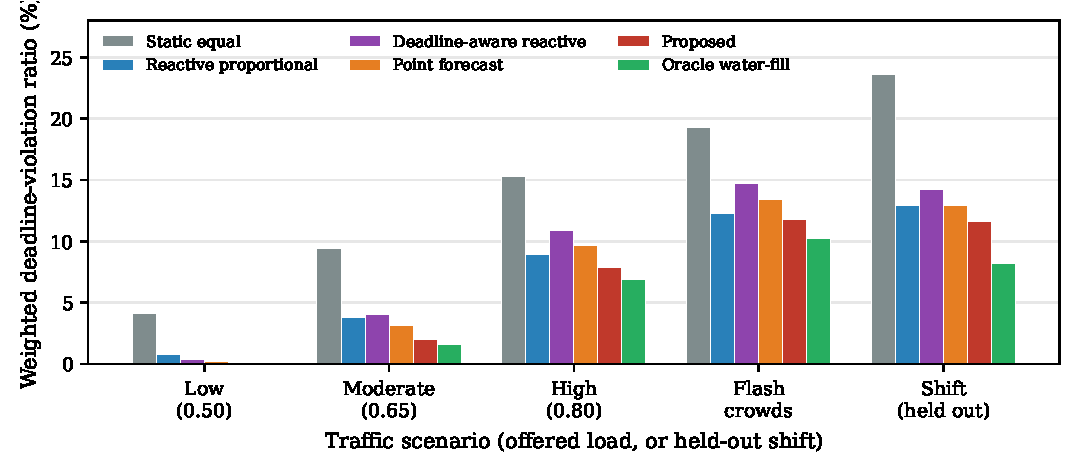
\includegraphics[width=0.98\linewidth]{figures/fig_violation.pdf}
\caption{Weighted violation ratio by scenario. The proposed rule is the lowest implementable bar in every group. The gap to the oracle remains visible at high load and under the shift.}
\label{fig:bars}
\end{figure}

Table~\ref{tab:main} and Fig.~\ref{fig:bars} are the main comparison. Against the point-forecast controller, which uses the same model but only the median, the proposed rule is lower on all five seeds in every scenario. The relative reductions are 53\%, 36\%, 18\%, 12\%, and 10\% from the low load through the shift. These are relative changes, \((v_{\mathrm{base}}-v_{\mathrm{prop}})/v_{\mathrm{base}}\), not percentage-point gaps. Against the deadline-aware reactive controller the corresponding reductions are 79\%, 51\%, 27\%, 20\%, and 18\%, again on every seed. The window-quantile variant, with no trained model, already beats both of those baselines; the trained quantiles add a further 51\% relative reduction at low load but only about 2\% under the shift. Most of the gain over the reactive baselines is therefore the demand definition and the split in~\eqref{eq:kkt}, not the learner.

\begin{figure}[t]
\centering
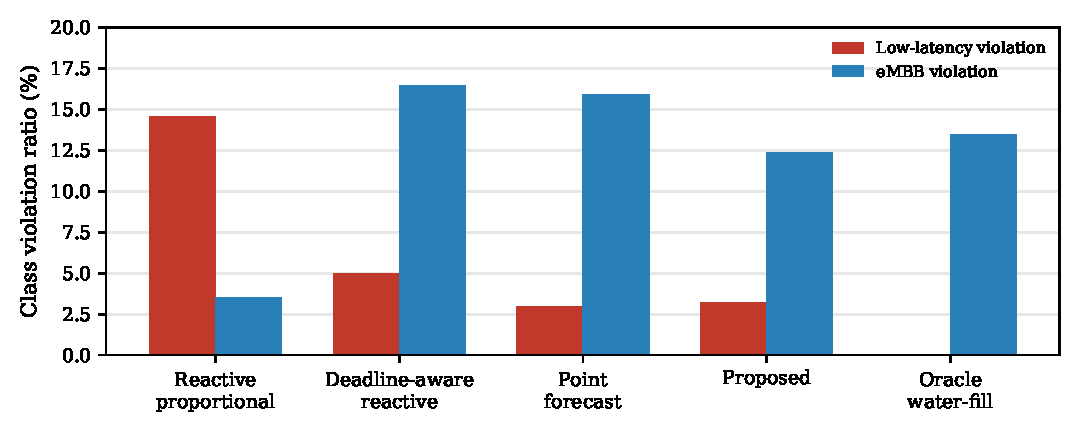
\includegraphics[width=0.92\linewidth]{figures/fig_classes.pdf}
\caption{High-load class violations (means over five seeds). Deadline-aware controllers protect the low-latency cells and spend eMBB bits. Among them, the proposed rule has the smallest eMBB loss.}
\label{fig:class}
\end{figure}

Figure~\ref{fig:class} shows where the high-load gain sits. Reactive proportional keeps eMBB loss at 3.5\% but drops 14.6\% of low-latency bits. Deadline-aware reactive and the point forecast cut low-latency loss to about 5.0\% and 3.0\%, at an eMBB loss of 16.4\% and 15.9\%. The proposed rule holds low-latency loss at 3.2\% and eMBB loss at 12.3\%, with utilisation 72.0\% against 70.0\% for the point forecast and 69.2\% for deadline-aware reactive. The oracle still loses 13.4\% of eMBB bits: a budget frozen for 10~ms cannot follow every burst. Jain's index of the per-cell service ratio exceeds 0.99 for every controller and does not separate them. Mean DU queueing delay at high load is about 4.2~ms for the proposed rule. The 99th percentile sits on the 10~ms eMBB deadline for all methods, so it is not informative. Calibration increased the weighted ratio, by about 10\% relative under the shift, because low-latency misses caused by the shared shortage were treated as forecast bias and the low-latency cells then over-reserved.

Two further sweeps bound the regime. On the high-load interval sweep (three seeds, forecasters retrained at each interval), the proposed rule at \(T=4\) slots is 62\% below deadline-aware reactive, 27\% below reactive proportional, and 57\% below the oracle water-fill. At \(T=40\) slots it is 12\% \emph{above} reactive proportional: reserving a short-deadline peak for 20~ms wastes the link. A separate moderate-load sweep changes only the mantissa width, hence \(\beta\), on identical user traffic (three seeds). At 6, 9, 12, and 14 bits the realised loads are 0.43, 0.63, 0.83, and 0.97, and the proposed weighted ratios are 0.04\%, 1.60\%, 10.8\%, and 19.3\%. Reactive proportional is 0.13\%, 3.43\%, 10.7\%, and 16.4\%. Allocation helps in the middle of that range. Near a full link, protecting low-latency traffic costs more weighted eMBB loss than it saves, and the proportional controller is better. This sweep does not model the signal-quality cost of a narrower mantissa.

A separate CPU benchmark times matrix inversion on synthetic well-conditioned matrices \(A=G/\sqrt{n}+2I\), with 200 held-out matrices per size. It was not re-timed for this report; the times below are the saved medians. LAPACK inversion takes 0.17~ms at \(n=100\) and 18~ms at \(n=500\), with relative error near \(5\times 10^{-8}\). A direct multilayer perceptron has relative error 0.36 at \(n=10\) and 0.52 at \(n=100\), so it is not an inverse. A learned Newton--Schulz iteration~\cite{schulz1933} reaches relative error \(1.4\times 10^{-6}\) at \(n=100\) and \(n=500\), but its median time (0.46~ms and 34~ms) does not beat LAPACK. At \(n=10\) that learned iteration is inaccurate (relative error 0.17). A \(0.5\,\mathrm{ms}\) slot can hold the saved \(n=100\) LAPACK median on that host; the \(n=500\) median does not fit one slot. These are single-matrix CPU times, not a fronthaul scheduler.

\subsection{Current status and limitations}

The allocation simulator, the quantile forecaster, the baselines, the tests, and the saved logs are implemented and, for the high-load table, reproduced. The evidence is five seeds of synthetic traffic on one topology. Absolute violation levels are high because the bursts are heavy-tailed and the budget is held for 10~ms; even the oracle loses a large eMBB fraction. The method is not uniformly best: it ties with reactive proportional under flash crowds (three of five seeds, about 3\% relative), loses to it at a 20~ms interval and at offered load 0.97, and gains little from the trained model under the shift. Decision time for the proposed rule was about 3.5~ms per 10~ms epoch in Python on this host, almost all of it in the trees. That does not establish operation inside a radio scheduler. Earlier I/Q compression figures exist in the repository, but the encoder sources they depend on are absent from the tree that contains \texttt{fhlm}, so those curves are not reported as results here.

\section{Planned Workflow and Timeline}

The end-semester evaluation is expected around the last week of November 2026. No exact date is treated as fixed. The next technical milestone is a sensitivity check of \(T\), \(\tau\), and the priority weights on the same simulator, with the raw logs stored beside the present results.

\begin{table}[h]
\centering
\caption{Remaining work from this report through the end-semester period.}
\label{tab:plan}
\small
\setlength{\tabcolsep}{3.5pt}
\begin{tabular}{@{}p{2.5cm}p{5.4cm}p{6.6cm}@{}}
\toprule
Window & Task and deliverable & Dependency \\
\midrule
29 Sep--10 Oct &
Sensitivity of \(T\), \(\tau\), and weights; a short note of where the ranking changes. &
Present simulator and test seeds. \\
13--24 Oct &
Restore a re-runnable compression path and connect mantissa width to NMSE, or drop that claim. &
Missing encoder sources. \\
27 Oct--7 Nov &
More seeds on the high and shift scenarios; state win counts only. &
Compute time on a CPU host. \\
10--18 Nov &
Supervisor review of the draft end-semester report and the result tables. &
Review comments. \\
19--26 Nov &
Final report, plagiarism check, and presentation. &
Department instructions. \\
\bottomrule
\end{tabular}
\end{table}

At mid-semester the shared-link rule and its main comparison are in place, including the cases where it does not win. The immediate milestone is the sensitivity note, not a new algorithm and not an over-the-air trial, for which this repository has no radio setup.

\enlargethispage{2\baselineskip}
\begin{thebibliography}{99}
\bibitem{oran-cus}
O-RAN Alliance WG4, ``Control, User and Synchronization Plane Specification,'' O-RAN.WG4.CUS, including the 7-2x user plane and block-floating-point annex.
\bibitem{larsen2019}
L.~M.~P. Larsen, A.~Checko, and H.~L. Christiansen, ``A survey of the functional splits proposed for 5G mobile crosshaul networks,'' \emph{IEEE Commun.\ Surveys Tuts.}, vol.~21, no.~1, pp.~146--172, 2019, doi: 10.1109/COMST.2018.2868805.
\bibitem{wang2017}
L.~Wang and S.~Zhou, ``On the fronthaul statistical multiplexing gain,'' \emph{IEEE Commun.\ Lett.}, vol.~21, no.~5, pp.~1099--1102, 2017, doi: 10.1109/LCOMM.2017.2653120.
\bibitem{perez2018}
G.~O. P\'erez, J.~A. Hern\'andez, and D.~Larrabeiti, ``Fronthaul network modeling and dimensioning meeting ultra-low latency requirements for 5G,'' \emph{J.\ Opt.\ Commun.\ Netw.}, vol.~10, no.~6, pp.~573--581, 2018, doi: 10.1364/JOCN.10.000573.
\bibitem{lagen2022}
S.~Lag\'en, X.~Gelabert, A.~Hansson, M.~Requena, and L.~Giupponi, ``Fronthaul compression control for shared fronthaul access networks,'' \emph{IEEE Commun.\ Mag.}, 2022, doi: 10.1109/MCOM.001.2100959.
\bibitem{bega2020}
D.~Bega, M.~Gramaglia, M.~Fiore, A.~Banchs, and X.~Costa-P\'erez, ``AZTEC: Anticipatory capacity allocation for zero-touch network slicing,'' in \emph{Proc.\ IEEE INFOCOM}, 2020, doi: 10.1109/INFOCOM41043.2020.9155299.
\bibitem{cohen2023}
K.~M. Cohen, S.~Park, O.~Simeone, P.~Popovski, and S.~Shamai, ``Guaranteed dynamic scheduling of ultra-reliable low-latency traffic via conformal prediction,'' \emph{IEEE Signal Process.\ Lett.}, vol.~30, pp.~473--477, 2023, doi: 10.1109/LSP.2023.3264939.
\bibitem{leboudec2001}
J.-Y. Le~Boudec and P.~Thiran, \emph{Network Calculus}. Springer, 2001.
\bibitem{hadley1963}
G.~Hadley and T.~M. Whitin, \emph{Analysis of Inventory Systems}. Prentice-Hall, 1963.
\bibitem{gibbs2021}
I.~Gibbs and E.~Cand\`es, ``Adaptive conformal inference under distribution shift,'' in \emph{Advances in Neural Information Processing Systems}, 2021.
\bibitem{willinger1997}
W.~Willinger, M.~S. Taqqu, R.~Sherman, and D.~V. Wilson, ``Self-similarity through high-variability: Statistical analysis of Ethernet LAN traffic at the source level,'' \emph{IEEE/ACM Trans.\ Netw.}, vol.~5, no.~1, pp.~71--86, 1997.
\bibitem{schulz1933}
G.~Schulz, ``Iterative Berechnung der reziproken Matrix,'' \emph{Z.\ Angew.\ Math.\ Mech.}, vol.~13, no.~1, pp.~57--59, 1933.
\end{thebibliography}

\end{document}
